\documentclass{book}
\usepackage{physics}
\usepackage{graphicx}
\usepackage{caption}
\usepackage{amsmath}
\usepackage{bm}
\usepackage{framed}
\usepackage{authblk}
\usepackage{empheq}
\usepackage{amsfonts}
\usepackage{esint}
\usepackage[makeroom]{cancel}
\usepackage{dsfont}
\usepackage{centernot}
\usepackage{mathtools}
\usepackage{bigints}
\usepackage{amsthm}
\theoremstyle{definition}
\newtheorem{defn}{Definition}[section]
\newtheorem{prop}{Proposition}[section]
\newtheorem{rmk}{Remark}[section]
\newtheorem{thm}{Theorem}[section]
\newtheorem{exmp}{Example}[section]
\newtheorem{prob}{Problem}[section]
\newtheorem{sln}{Solution}[section]
\newtheorem*{prob*}{Problem}
\newtheorem{exer}{Exercise}[section]
\newtheorem*{exer*}{Exercise}
\newtheorem*{sln*}{Solution}
\usepackage{empheq}
\usepackage{hyperref}
\usepackage{tensor}
\usepackage{xcolor}
\hypersetup{
	colorlinks,
	linkcolor={black!50!black},
	citecolor={blue!50!black},
	urlcolor={blue!80!black}
}


\newcommand*\widefbox[1]{\fbox{\hspace{2em}#1\hspace{2em}}}

\newcommand{\p}{\partial}
\newcommand{\R}{\mathbb{R}}
\newcommand{\C}{\mathbb{C}}
\newcommand{\lag}{\mathcal{L}}
\newcommand{\nn}{\nonumber}
\newcommand{\had}{\mathcal{H}}
\newcommand{\M}{\mathcal{M}}
\newcommand{\I}{\mathcal{I}}
\newcommand{\K}{\mathcal{K}}
\newcommand{\F}{\mathcal{F}}
\newcommand{\w}{\omega}
\newcommand{\lam}{\lambda}
\newcommand{\al}{\alpha}
\newcommand{\be}{\beta}
\newcommand{\x}{\xi}

\newcommand{\G}{\mathcal{G}}

\newcommand{\f}[2]{\frac{#1}{#2}}

\newcommand{\ift}{\infty}

\newcommand{\lp}{\left(}
\newcommand{\rp}{\right)}

\newcommand{\lb}{\left[}
\newcommand{\rb}{\right]}

\newcommand{\lc}{\left\{}
\newcommand{\rc}{\right\}}


\newcommand{\V}{\mathbf{V}}
\newcommand{\U}{\mathcal{U}}
\newcommand{\Id}{\mathcal{I}}
\newcommand{\D}{\mathcal{D}}
\newcommand{\Z}{\mathcal{Z}}

%\setcounter{chapter}{-1}


\makeatletter
\renewcommand{\@chapapp}{Part}
%\renewcommand\thechapter{$\bf{\ket{\arabic{chapter}}}$}
%\renewcommand\thesection{$\bf{\ket{\arabic{section}}}$}
%\renewcommand\thesubsection{$\bf{\ket{\arabic{subsection}}}$}
%\renewcommand\thesubsubsection{$\bf{\ket{\arabic{subsubsection}}}$}
\makeatother



\usepackage{subfig}
\usepackage{listings}
\captionsetup[lstlisting]{margin=0cm,format=hang,font=small,format=plain,labelfont={bf,up},textfont={it}}
\renewcommand*{\lstlistingname}{Code \textcolor{violet}{\textsl{Mathematica}}}
\definecolor{gris245}{RGB}{245,245,245}
\definecolor{olive}{RGB}{50,140,50}
\definecolor{brun}{RGB}{175,100,80}
\lstset{
	tabsize=4,
	frame=single,
	language=mathematica,
	basicstyle=\scriptsize\ttfamily,
	keywordstyle=\color{black},
	backgroundcolor=\color{gris245},
	commentstyle=\color{gray},
	showstringspaces=false,
	emph={
		r1,
		r2,
		epsilon,epsilon_,
		Newton,Newton_
	},emphstyle={\color{olive}},
	emph={[2]
		L,
		CouleurCourbe,
		PotentielEffectif,
		IdCourbe,
		Courbe
	},emphstyle={[2]\color{blue}},
	emph={[3]r,r_,n,n_},emphstyle={[3]\color{magenta}}
}


\begin{document}
\begin{titlepage}\centering
 \clearpage
 \title{{\textsc{\textbf{Physics at the Perimeter Institute:\\  Topics in Theoretical Physics \\ 
 				\&\\ Quantum Simulation Research}}}\\ \smallskip - A Quick Guide - \\}
 \author{\bigskip Huan Q. Bui}
  \affil{Colby College\\$\,$\\ PHYSICS \& MATHEMATICS\\ Statistics \\$\,$\\Class of 2021\\}
 \date{\today}
 \maketitle
 \thispagestyle{empty}
\end{titlepage}

\subsection*{Preface}
\addcontentsline{toc}{subsection}{Preface}

Greetings,\\

This guide is my notes from Perimeter Institute of Theoretical Physics Summer School, 2020. Topics include quantum information, thermodynamics, numerical methods, condensed matter physics, path integrals, and symmetries.\\

Enjoy!  



\newpage
\tableofcontents
\newpage





\chapter{Quantum Information \& Thermodynamics} 

The aim of this course is to understand the thermodynamics of quantum systems and in the process to learn some fundamental tools in Quantum Information. We will focus on the topics of foundations of quantum statistical mechanics, resource theories, entanglement, fluctuation theorems, and quantum machines. 

\newpage

\section{Foundations of Quantum Statistical Mechanics - Entanglement}
\newpage

\section{Resource Theories and Quantum Information}


\newpage
\section{Quantum Thermal Operations}


\newpage
\section{Fluctuation Theorems and Quantum Information}


\newpage
\section{Quantum Thermal Machines}






\newpage
\chapter{Numerical Methods \& Condensed Matter Physics}

This course has two main goals: (1) to introduce some key models from condensed matter physics; and (2) to introduce some numerical approaches to studying these (and other) models.  As a precursor to these objectives, we will carefully understand many-body states and operators from the perspective of condensed matter theory.  (However, I will cover only spin models.  We will not discuss or use second quantization.)\\



Once this background is established, we will study the method of exact diagonalization and write simple python programs to find ground states, correlation functions, energy gaps, and other properties of the transverse-field Ising model and XXZ model.  We will also discuss the computational limitations of exact diagonalization.  Finally, I will introduce the concept of matrix product states, and we will see how these can be used with algorithms such as the density matrix renormalization group (DMRG) to study ground state properties for much larger systems than can be studied with exact diagonalization.




\newpage

\section{Lecture 1}
\subsection{Introduction to many-particle states and operators}
\newpage
\subsection{Introduction to Ising and XXZ models}
\newpage
\subsection{Programming basics}
\newpage
\subsection{Finding expectation values}
\newpage

\section{Lecture 2: Exact diagonalization part 1}
\subsection{Representing models}
\newpage
\subsection{Finding eigenstates}
\newpage
\subsection{Energy gaps}
\newpage
\subsection{Phase transitions}
\newpage




\section{Lecture 3: Exact diagonalization part 2}
\subsection{Limitations of the method}
\newpage
\subsection{Using symmetries}
\newpage
\subsection{Dynamics}
\newpage




\section{Lecture 4: Matrix product states part 1}
\subsection{Entanglement and the singular value decomposition}
\newpage
\subsection{What is a matrix product state and why is it useful}
\newpage


\section{Lecture 5: Matrix product states part 2}
\subsection{Algorithms for finding ground states using matrix product states: iTEBD }

\newpage


\subsection{Algorithms for finding ground states using matrix product states: DMRG }

\newpage











\chapter{Path Integrals}

The goal of this course is to introduce the path integral formulation of quantum mechanics and a few of its applications. We will begin by motivating the path integral formulation and explaining its connections to other formulations of quantum mechanics and its relation to classical mechanics. We will then explore some applications of path integrals.


\newpage

\section{Introduction to path integrals and the semi-classical limit}

\newpage
\section{Propagator in real and imaginary time}


\newpage

\section{Perturbation theory}


\newpage

\section{Non-perturbative physics and quantum tunneling}


\newpage


\section{Topology and path integrals}


\newpage



\chapter{Symmetries}



The aim of this course is to  explore some of the many ways in which symmetries play a role in physics. We’ll start with an overview of the concept of symmetries and their description in the language of  group theory. We will then discuss continuous symmetries and infinitesimal symmetries, their fundamental role in Noether's theorem, and their formalization in terms of Lie groups and Lie algebras. In the last part of the course we will focus on symmetries in quantum theory and introduce representations of (Lie) groups and Lie algebras.


\newpage

\section{Lecture 1: Overview}
\subsection{Definition of symmetry}
\newpage
\subsection{Elements of group theory}
\newpage
\subsection{Examples }
\newpage



\section{Lecture 2}
\subsection{Continuous and discrete symmetries}
\newpage
\subsection{Infinitesimal symmetries}
\newpage
\subsection{Noether's theorem}


\newpage

\section{Lecture 3: Lie groups and Lie algebras}
\newpage

\section{Lecture 4: Symmetries in quantum mechanics}
\newpage
\section{Representation theory}



\newpage



\chapter{Research Project: Quantum Simulation}

\textbf{Quantum many-body physics on quantum hardware}\\


\underline{Project description:} Recently, there have been significant advances in several quantum computing platforms, including superconducting qubits and trapped ions. At this point, nontrivial quantum operations can be implemented
on tens of qubits, and the frontier continues to expand. This project will explore how these emerging
technologies can assist the realization and understanding of complex many-body quantum systems,
regarding both static aspects such as ground state properties and dynamical aspects such as quantum chaos
and thermalization. What new physics can we learn from near-term quantum computers? The ideal
outcome is an interesting and realistic proposal that can be carried out in one of the quantum platforms (see
for example the interplay between theoretical proposals and experiment).














\newpage


\section{Review: The density operator}


We often use the language of state vectors in quantum mechanics. An alternative language is that of \textit{density matrices/density operators}. We will use this language extensively in quantum information/quantum computation. First, we will introduce the formulation. Second, we look at some properties of the density operator. Finally, we look at an application where the density operator really shines -- as a tool for describing \textit{individual subsystems} of a composite quantum system.  


\subsection{Ensembles of Quantum States}

The density operator language provides a convenient means for describing quantum systems whose state is not completely known. Suppose a quantum system is in one of the states $\ket{\psi_i}$ where $i$ is an index, with respective probabilities $p_i$. We call $\{p_i, \ket{\psi_i}\}$ an \textit{ensemble of pure states}. \\

\begin{defn}[Density Operator]
	\begin{align}
	\boxed{\rho \equiv \sum_i p_i \ket{\psi_i}\bra{\psi_i}}
	\end{align}
\end{defn}



Suppose we let a unitary $\U$ act on a closed system. If the system was initially in the state $\ket{\psi_i}$ with probability $p_i$ then we get $\U \ket{\psi_i}$ with probability $p_i$. The density operator evolves as
\begin{align}
\rho = \sum_i p_i \ket{\psi_i}\bra{\psi_i} \stackrel{\U}{\rightarrow} \sum_i p_i \U \ket{\psi_i}\bra{\psi_i}\U^\dagger = \U \rho \U^\dagger.
\end{align}


Suppose we have a measurement gate $\M_m$. If the intial state is $\ket{\psi_i}$ then the probability of getting result $m$ is 
\begin{align}
p(m\vert i) = \bra{\psi_i} \M_m^\dagger \M_m \ket{\psi_i} = \tr\lp \M_m^\dagger \M_m \braket{\psi_i} \rp
\end{align}
where we have used the identity:
\begin{align}
\tr(A\ket{\psi}\bra{\psi}) = \sum_i \bra{i}A \ket{\psi}\bra{\psi}\ket{i} = \bra{\psi}A\ket{\psi}.
\end{align}
With this, the total probability of measuring $m$ is 
\begin{align}
p(m) = \sum_i p(m|i)p_i = \sum_i p_i \tr\lp \M_m^\dagger \M_m \ket{\psi_i}\bra{\psi_i} \rp = \tr\lp \M_m^\dagger \M_m \rho \rp.
\end{align}

The state after the measurement is thus
\begin{align}
\ket{\psi_i^m} = \f{\M_m \ket{\psi_i}}{\sqrt{\bra{\psi_i}\M_m^\dagger \M_m \ket{\psi_i}}}.
\end{align}
The corresponding density operator for this state is thus
\begin{align}
\rho_m = \sum_i p(i|m)\ket{\psi_i^m}\bra{\psi_i^m} = \sum_i p(i|m)\f{\M_m \ket{\psi_i}\bra{\psi_i}\M_m^\dagger}{\bra{\psi_i}\M_m^\dagger \M_m \ket{\psi_i}}.
\end{align}
From probability theory we have $p(i|m) = p(m|i)p_i/p(m)$, so:
\begin{align}
\rho_m = \sum_i p_i \f{\M_m \ket{\psi_i}\bra{\psi_i}\M_m^\dagger}{\tr\lp \M^\dagger_m \M_m \rho \rp} = \f{\M_m \rho \M_m^\dagger}{\tr\lp \M_m^\dagger \M_m \rho \rp}.
\end{align}




Finally, suppose we have a quantum system in state $\rho_i$ with probability $p_i$. The system might be described by the density matrix
\begin{align}
\rho = \sum_i p_i \rho_i.
\end{align}
Here's why:
\begin{align}
\rho = \sum_{i,j}p_i p_{ij}\ket{\psi_{ij}}\bra{\psi_{ij}} = \sum_i p_i \rho_i
\end{align}
where we have used the definition
\begin{align}
\rho_i = \sum_{j}p_{ij}\ket{\psi_{ij}}\bra{\psi_{ij}}.
\end{align}

We call $\rho$ the \textit{mixture} of the states $\rho_i$ with probabilities $p_i$. This concept of mixture comes up up repeatedly in the analysis of problems like quantum noise, where the effect of the noise is to introduce ignorance into our knowledge of the quantum state. A simple example is provided by the measurement scenario. Imagine that for some reason out record of the result $m$ of the measurement was lost. We would have a quantum system in the state $\rho_m$ with probability $p(m)$, but would no longer know the actual value of $m$. The state of such a quantum system would therefore by described by the density operator
\begin{align}
\rho = \sum_m p(m)\rho_m = \sum_m \tr\lp \M_m^\dagger \M_m \rho \rp\f{\M_m \rho \M_m^\dagger}{\tr\lp \M_m^\dagger \M_m \rho \rp} = \sum_m \M_m \rho \M_m^\dagger.
\end{align}






























\subsection{General Properties of the Density Operator}



\begin{thm}[Characterization of density operators] 
	An operator $\rho$ is the density operator to some ensemble $\{p_i, \ket{\psi_i} \}$ if and only if it statisfies the conditions
	\begin{itemize}
		\item \textbf{Trace condition:} $\tr(\rho) = 1$.
		\item \textbf{Positivity:} $\rho$ is a positive operator, i.e., $\bra{\varphi}\rho\ket{\varphi} \geq 0 \forall \varphi$.
	\end{itemize}
\end{thm}


With this definition we can reformulate the postulates of quantum mechanics in the language of density operators as 
\begin{itemize}
	\item \textbf{Postulate 1:} Associated to any isolated physical system is a Hilbert space known as the \textit{state space} of the system. The system is completely described by its \textit{density operator}, which is a positive operator $\rho$ with trace one, acting on the state space of the system. If a quantum system is in the state $\rho_i$ with probability $p_i$ then the density operator for the system is $\sum _i p_i \rho_i$.
	
	\item \textbf{Postulate 2:} The evolution of a \textit{closed} quantum system is described by a \textit{unitary transformation}:
	\begin{align}
	\rho' = \U \rho \U^\dagger.
	\end{align} 
	
	
	
	\item \textbf{Postulate 3:} Measurements are described by a collection $\{\M_m\}$ of \textit{measurement operators}. The index $m$ refers to the measurement outcomes that may occur. If the state of the quantum system is $\rho$ immediately before the measurement then the probability that result $m$ occurs is given by
	\begin{align}
	p(m) = \tr\lp \M_m^\dagger  \M_m \rho_m \rp
	\end{align}
	and the state of the system after the measurement is 
	\begin{align}
	\f{\M_m \rho \M_m^\dagger}{\tr\lp \M_m^\dagger \M_m \rho \rp}.
	\end{align}
	The measurement operators satisfy the completeness equation
	\begin{align}
	\sum_m \M_m^\dagger \M_m = \Id.
	\end{align}
	
	
	
	\item \textbf{Postulate 4:} The state space of a composite physical system is the tensor product of the state spaces of the component physical systems. E.g. the joint state of the total system can be written as $\rho_1 \otimes \dots \otimes \rho_n$.
\end{itemize}



\begin{thm}[Pure states] 
	$\tr(\rho^2) \leq 1$. Equality occurs if and only if $\rho$ is a pure state. 
\end{thm}



\begin{thm}[Unitary freedom in the ensemble for density matrices] 
	The sets $\ket{\tilde{\varphi}_i}$ and $\ket{\tilde{\psi}_j}$ generate the same density matrix if and only if they are unitarily similar, i.e., 
	\begin{align}
	\ket{\tilde{\varphi}_i} = \sum_{j} u_{ij}\ket{\tilde{\psi}_j}
	\end{align}
	where the $u_{ij}$ are entries of a unitary $\U$.
	
\end{thm}




\subsection{The Reduced Density Operator}
Te deepest application of the density operator is as a descriptive tool for \textit{sub-systems} of a composite quantum system. Such a description is given by the \textit{reduced density operator}. \\

Suppose we have physical systems $A$ and $B$ whose state is described by the density operator $\rho^{AB}$. The reduced density operator for $A$ is then given by
\begin{align}
\rho^A = \tr_B\lp \rho^{AB} \rp
\end{align}
where $\tr_B$ is the \textit{partial trace} over system $B$, defined by
\begin{align}
\tr_B\lp \ket{a_1}\bra{a_2} \otimes \ket{b_1}\bra{b_2} \rp \equiv \ket{a_1}\bra{a_2}\tr\lp \ket{b_1}\bra{b_2} \rp = \ket{a_1}\bra{a_2}\braket{b_2}{b_1}
\end{align}
where $\ket{a_1}, \ket{a_2}$ are any two vectors in the state space of $A$, and $\ket{b_1}, \ket{b_2}$ are any two vectors in the state space of $B$. \\




\begin{exmp}
	To understand this construction, consider an example where $\rho^{AB} = \rho \otimes \sigma$ where $\rho,\sigma$ describe $A,B$ respectively. Then
	\begin{align}
	\rho^A = \tr_B\lp \rho \otimes \sigma \rp = \rho \tr(\sigma) = \rho
	\end{align}
	as expected. 
\end{exmp}











\newpage






\section{Quantum Simulation: A Primer}


\subsection{Simulation in action}
\subsection{The quantum simulation algorithm}
\subsection{An illustrative example}
\subsection{Perspectives on quantum simulation}



\newpage



\section{Quantum Phase Estimation (QPE)}

One of the most important applications of the Quantum Fourier Transform is the Quantum Phase Estimation. Phase estimation is the key for many quantum algorithms. Suppose a unitary operator $\U$ has an eigenvector $\ket{u}$ with eigenvalue $2^{2\pi i \varphi}$, where the value of $\varphi$ is unknown. The goal of the phase estimation algorithm is to estimate $0 \leq \varphi \leq 1$ with high probability within additive error $\epsilon$. The algorithm uses $\mathcal{O}(\log (1/\epsilon))$ qubits and $\mathcal{O}(1/\epsilon)$ controlled-$\U$ operations. \\

To perform the estimation we assume that we have available \textit{oracles} capable of preparing the state $\ket{u}$ (the eigenstate) and performing the controlled-$\U^{2j}$ operation, for suitable nonnegative integers $j$. Since preparing eigenstates is not necessarily easy, the phase estimation algorithm is not a complete algorithm by itself. Rather, we should view it as a ``subroutine'' or a ``module.''\\



The QPE uses two registers. The first register contains $t$ qubits initially in $\ket{0}$. The choice of $t$ depends on two things: the number of digits of accuracy we wish to have in our estimate of $\varphi$, and with what probability we wish the phase estimation procedure to be successful. The second register begins in the eigenstate $\ket{u}$, and contains as many qubits as necessary to store $\ket{u}$. \\

QPE occurs in two main stages. First, the circuit applies  an $\had$ to each of the $t$ qubits. Then, the circuit applies controlled-$\U$ operators on the second register, with $\U$ raised to successive powers of two. This stage looks like the following:
\begin{figure}[!htb]
	\centering
	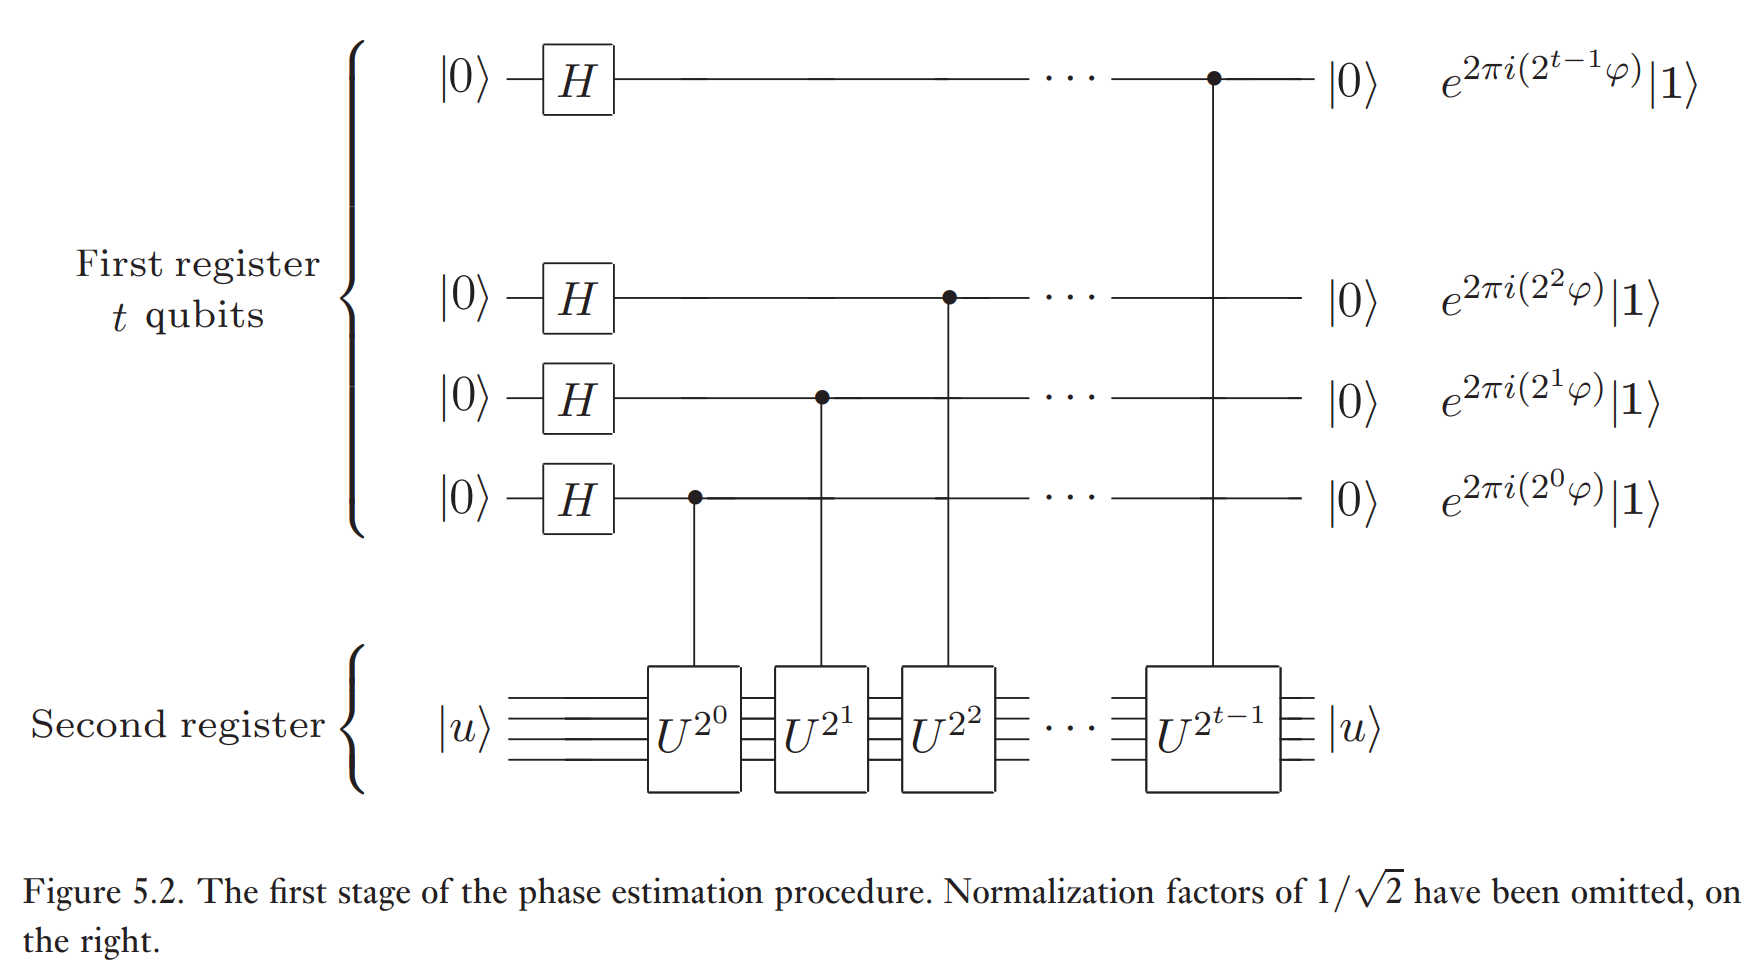
\includegraphics[scale=0.25]{qpe1}
	\caption{Source: Mike and Ike}
\end{figure} 
Recall that immediately after $\had^{\otimes t}$ the state of the upper register looks like
\begin{align}
\had \ket{0} = \f{1}{2^{1/2}}\lp \ket{0} + \ket{1} \rp
\end{align}
The controlled-$\U$ acts on $\ket{u}$ only if the control qubit is in $\ket{1}$. With this, we see that the final state of the first register is given by
\begin{align}
&\f{1}{2^{t/2}}\lp \ket{0} + e^{2\pi i 2^{t-1}\varphi}\ket{1} \rp\otimes
\lp \ket{0} + e^{2\pi i 2^{t-2}\varphi}\ket{1} \rp \otimes \dots \otimes \lp \ket{0} + e^{2\pi i 2^{0}\varphi}\ket{1} \rp\nn\\
&\quad = \dots \nn\\
&\quad = \f{1}{2^{t/2}}\sum_{0\leq k < 2^{t}} e^{2\pi i \varphi k}\ket{k}_t.
\end{align}

\begin{exmp}
For $t =2$, we have
\begin{align}
&\f{1}{2}\lp \ket{0} + e^{4\pi i \varphi } \ket{1} \rp\otimes \lp \ket{0} + e^{2\pi i\varphi }\ket{1} \rp \nn\\
&\quad= \f{1}{2}\lp \ket{0}_2 + e^{1\cdot 2\pi i\varphi }\ket{1}_2 + e^{2\cdot 2\pi i\varphi}\ket{2}_2 + e^{3\cdot 2\pi i\varphi }\ket{3}_2  \rp\nn\\
&\quad = \f{1}{2^{2/2}}\sum_{0 \leq k < 2^{2}}e^{2\pi i \varphi \cdot 2}\ket{k}_2
\end{align}\qed
\end{exmp}

Note that we're leaving out the qubits carrying the  $\ket{u}$ state because we don't do anything to it (because $\ket{u}$ is an eigenstate of $\U$). We should also note that the effect of the sequence of controlled-$\U$ operations is to take $\ket{j}\ket{u}$ to $\ket{j}\U^j \ket{u}$. We should also note that this does not depend on the fact that $\ket{u}$ is an eigenstate of $\U$. \\


In the second state, the algorithm applies the inverse quantum Fourier transform on the first register (which is just the QFT, applied in reverse order of operations). This can be done efficiently in $\mathcal{O}(t^2)$ steps, as we have seen the Quantum Information \href{https://huanqbui.com/LaTeX 20projects/HuanBui_QI/HuanBui_QI.pdf}{\underline{notes}}. Since the input in this case is the maximal superposition in the $t$-vector space, the output of the inverse QFT is going to be a single state: $\ket{\tilde{\varphi}}$, which we hope is approximately $\ket{\varphi}$. We will see how close $\ket{\tilde\varphi}$ can get to $\ket{\varphi}$.\\

The third and final stage of the algorithm is to read out the state of the first register by doing a measurement in the computational basis. \\


\begin{exmp}
	To make sure we see what is going on, suppose $\varphi$ is expressed exactly in $t$ qubits, as $\varphi = 0,\varphi_1\varphi-2\dots\varphi_t$ (note that $\varphi \in [0,1]$). Then the state of the input register after the first stage is given by
	\begin{align}
	\f{1}{2^{t/2}}\lp \ket{0} + e^{2\pi i 0.\varphi_t} \ket{1} \rp \otimes \lp \ket{0} + e^{2\pi i 0.\varphi_{t-1}\varphi_t}\ket{1} \rp \otimes \dots  \otimes \lp \ket{0} + e^{2\pi i 0.\varphi_1\varphi_2\dots\varphi_t}\ket{1} \rp.
	\end{align}
	Applying the inverse QFT to this, we see that output state from the second state is the product state $\ket{\varphi_1\dots \varphi_t}$. A measurement in the computational basis gives $\varphi$ exactly. \qed
\end{exmp}

Schematically, the algorithm for QPE looks like the following:
\begin{figure}[!htb]
	\centering
	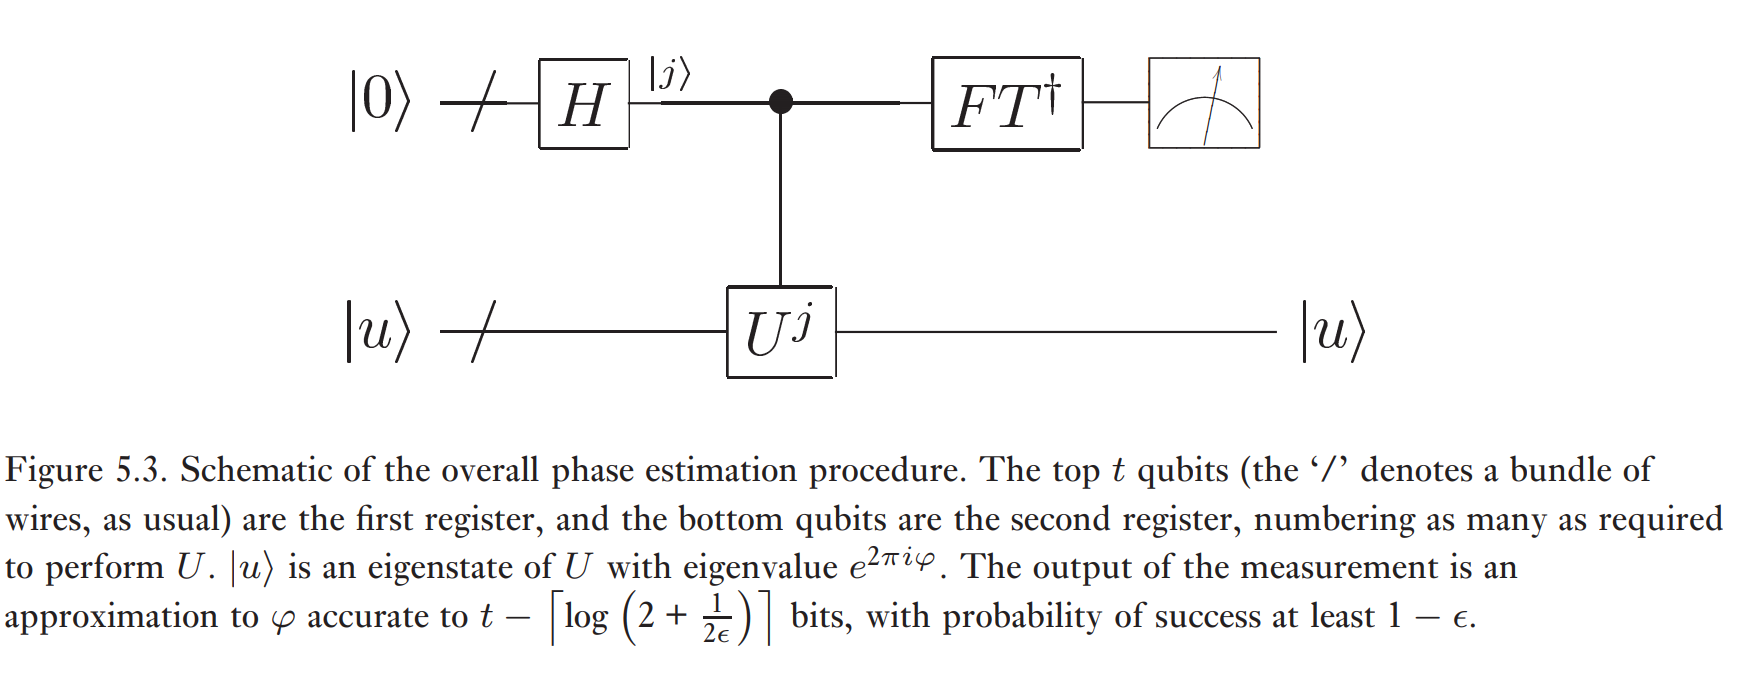
\includegraphics[scale=0.25]{qpe2}
	\caption{Source: Mike and Ike}
\end{figure}

In summary, what we basically did was using the inverse QFT to get
\begin{align}
\f{1}{2^{t/2}}\sum_{0 \leq k < 2^{t}} e^{2\pi i \varphi j }\ket{j}\ket{u} \to \ket{\tilde{\varphi}}\ket{u}
\end{align}
where $\ket{\tilde\varphi}$ is a good estimator for $\varphi$ when measured. 

 





\subsection{Performance and Requirements}
What happens when $\varphi$ cannot be written exactly with a $t$-bit expansion? We will now show that the procedure we described will produce a good approximation to $\varphi$ with high probability. \\

Let $b \in [0,2^t-1]$ an integer be given such that $b/2^t = 0.b_1b_2\dotsb_t$ is the best $t$ bit approximation to $\varphi$ which is less than $\varphi$, i.e., 
\begin{align}
0 \leq \delta \equiv \varphi - b/2^t \leq 2^{-t}.
\end{align}
(This is getting pretty close to an analysis proof -- because it \textit{is} an analysis proof.) Applying the inverse QFT to the state immediately after the first stage gives
\begin{align}
\mathcal{F}^{-1}\lb\f{1}{2^{t/2}}\sum_{0 \leq k < 2^t}e^{2\pi i \varphi k}\ket{k} \rb &= \f{1}{2^{t}} \sum_{0 \leq k,l < 2^t} e^{\f{-2\pi i kl}{2^t}}e^{2\pi i \varphi k}\ket{l}\nn\\
& = \f{1}{2^t}\sum_{0 \leq k,l < 2^t}\lp e^{2\pi i(\varphi- l/2^t)} \rp^k \ket{l}
\end{align}
by definition. Note that when $\varphi$ can be expressed using exactly $t$ bits we are reduced to the simpler version of the problem described above. \\

Let $\al_l$ be the amplitude of $\ket{(b+l) \mod 2^t}$, i.e., 
\begin{align}
\alpha_l \equiv \f{1}{2^t}\sum_{0 \leq k < 2^t} \lp e^{2\pi i (\varphi - (b+l)/2^t)} \rp^k.
\end{align}
This is a partial sum of a geometric series. It is straightforward to show that
\begin{align}
\alpha_l = \f{1}{2^t}\lp \f{1 - e^{2\pi i (2^t \varphi - (b+l))}}{1 - e^{2\pi i (\varphi - (b+l)/2^t)}} \rp = \f{1}{2^t}\lp \f{1 - e^{2\pi i (2^t \delta - l)}}{1 - e^{2\pi i (\delta - l/2^t)}} \rp.
\end{align}
Suppose the outcome of the final measurement is $m$. We want to bound the probability that $\abs{m-b} > \epsilon$ (where $\epsilon$ is the tolerance), i.e., we don't want the probably that $m$ is far from $b$ to be large. Well, the probability of observing such an $m$ is given by
\begin{align}
P(\abs{m-b} > \epsilon) = \sum_{-2^{t-1} < l \leq -(\epsilon+1)} \abs{\al_l}^2 + \sum_{e+1 \leq l \leq 2^{t-1}}\abs{\al_l}^2.
\end{align}
For any real $\theta$, we have $\abs{1 - \exp(i\theta)} \leq 2$, so 
\begin{align}
\abs{\al_l} \leq \f{2}{2^t \abs{1 - e^{2\pi i (\delta - l/2^)}}}.
\end{align}
Further, provided $-\pi \leq \theta \leq \pi$, we have $\abs{1 - \exp(i\theta)} \geq 2\abs{\theta}/\pi$. Also, when $-2^{t-1} < l \leq 2^{t-1}$ we have $-\pi \leq 2\pi (\delta - l/2^t) \leq \pi$, so we have
\begin{align}
\abs{\al_l} \leq \f{1}{2^{t+1}(\delta - l/2^t)}.
\end{align}
With this we have
\begin{align}
p(\abs{m-b} > \epsilon) &\leq \f{1}{4}\lp \sum_{l = -2^{t-1}+1}^{-(\epsilon+1)} \f{1}{(l - 2^t \delta)^2} + \sum^{2^{t-1}}_{l = \epsilon+1} \f{1}{(l - 2^t \delta)^2}  \rp\nn\\
&\leq \f{1}{4}\lp \sum_{l = -2^{t-1}+1}^{-(\epsilon+1)} \f{1}{(l - 1)^2} + \sum^{2^{t-1}}_{l = \epsilon+1} \f{1}{(l - 1)^2}   \rp, \quad 0 \leq 2^t\delta < 1\nn\\
&\leq \f{1}{2}\sum^{2^{t-1}-1}_{l=\epsilon} \f{1}{l^2}\nn\\
&\leq \f{1}{2}\int^{2^{t-1}-1}_{\epsilon-1} \f{1}{l^2}\,dl\nn\\
&= \f{1}{2(\epsilon-1)}.
\end{align}
Suppose we wish to approximate $\varphi$ to an accuracy $2^{-n}$, i.e., we choose $\epsilon = 2^{t-n}-1$. By using $t =n+p$ qubits, we see that the probability of obtaining an approximation correct to this accuracy is at least 
\begin{align}
1-\f{1}{2(\epsilon-1)} = 1 - \f{1}{2(2^p - 2)}.
\end{align}
So, to successfully obtain $\varphi$ accurate to $n$ bits with probability of success at least $1-\epsilon$ we choose 
\begin{align}
t = n + \left\lceil \log \lp 2 + \f{1}{2\epsilon} \rp \right\rceil.
\end{align}

Now here's a catch: to use QPE, we need the eigenstate $\ket{u}$. What if we don't know how to prepare such a state? Suppose that we prepare some other state $\ket{\psi}$ in place of $\ket{u}$. We can write
\begin{align}
\ket{\psi} = \sum_u c_u \ket{u}
\end{align}
where $\ket{u}$ are the eigenstates of $U$. Suppose the eigenstate $\ket{u}$ has the eigenvalue $e^{2\pi i \varphi_u}$. Running the QPE on $\ket{\psi}$ will give
\begin{align}
\ket{\psi} \stackrel{\mbox{QPE}}{\to} \sum_u c_u \ket{\tilde{\varphi_u}}\ket{u},
\end{align}
where $\tilde{\varphi_u}$ is an estimation for $\varphi_u$. Reading out the first register gives us a good approximation for $\varphi_u$, where $u$ is chosen at random with probability $\abs{c_n}^2$. This procedure allows us to avoid preparing a possibly unknown eigenstate, but at the cost of introducing some additional randomness into the algorithm. It turns out that if $t$ is chosen according to the minimization procedure above, then the probability for measuring $\varphi_u$ accurate to $n$ bits at the conclusion of the phase estimation algorithm is at least $\abs{c_u}^2(1-\epsilon)$.







\subsection{The algorithm}
QPE solves a problem which is both non-trivial and interesting from a physical point of view. It allows us to estimate the eigenvalue associated to a given eigenvector of a unitary operator. It turns our that other interesting problems can be reduced to phase estimation, which makes QPE particularly useful.\\

\underline{Here's the algorithm:}
\begin{itemize}
	\item \textbf{Inputs:} (1) An oracle which performs a controlled-$\U^j$ operation, (2) an eigenstate $\ket{u}$ of $\U$ with eigenvalue $e^{2\pi i \varphi_u}$, and (3) $t = n + \left\lceil \log \lp 2 + 1/2\epsilon \rp \right \rceil$ qubits initialized to $\ket{0}$.
	
	
	\item \textbf{Outputs:} An $n$-bit approximation $\tilde\varphi_u$ of $\varphi_u$. 
	
	\item \textbf{Runtime:} $\mathcal{O}(t^2)$ operations (due to th inverse QFT) and one call to controlled-$\U^j$ oracle. Succeeds with probability at least $1-\epsilon$. 
	
	\item \textbf{Procedure:} 
	\begin{itemize}
		\item  Initial state: $\ket{0}\ket{u}$
		
		\item Create superposition: $\to (1/2^{t/2})\sum_{0 \leq j < 2^t}\ket{j}\ket{u}$.
		
		
		\item Apply the oracle:\\ $\to(1/2^{t/2})\sum_{0 \leq j < 2^t}\ket{j}\U^j\ket{u} = (1/2^{t/2})\sum_{0 \leq j < 2^t}e^{2\pi i j\varphi_u}\ket{j}\ket{u}$
		
		
		\item Apply inverse QFT: $\to \ket{\tilde\varphi_u}\ket{u}$. 
		
		\item Measure the first register: $\to \tilde \varphi_u$.
	\end{itemize}
\end{itemize}


The algorithm has a wide range of applications, including order-finding and factorization. 










\newpage



\section{Quantum Expectation Estimation (QEE)}


In this and the following section we will be looking at two quantum algorithms that are alternatives/improvements to QPE. 


\newpage


\section{Quantum Variational Eigensolver (QVE)}


\newpage


\section{Quantum Approximate Optimization Algorithm (QAOA)}

\newpage





















\end{document}
